\section{Morphologischer Kasten f\"{u}r die Konzepte}
Im Folgenden werden die Teill\"{o}sungen des morphologischen Kastens erl\"{a}utert und mit Hilfe der Anforderungsliste bewertet. Grunds\"{a}tzlich unterscheiden sich die Teilfunktionen der Aerosolbereitstellung, dem Aerosol und der Sprungerzeugung.
\\\\
Die Aerosolbereitstellung erfolgt entweder durch einen Aerosolgenerator, welcher das Aerosol generiert oder einem Druckbeh\"{a}lter, gef\"{u}llt mit Aerosol. M\"{o}glich ist es auch einen Rauchentwickler oder einen bereits partikelbelasteten Raum, beispielsweise eine Sporthalle als Aerosolquelle zu nutzen.
\\\\
Ein Aerosolgenerator erzeugt ein langzeitstabiles Pr\"{u}faerosol mit einer Partikelgr\"{o}{\ss}enverteilung\cite{candle}. Der Massenstrom und die Partikelanzahlkonzentration sind regulierbar. Diese Konditionierung des Aerosols ist bei einer vorhandenen Aerosolquelle wie einem gef\"{u}llten Druckbeh\"{a}lter oder einem Rauchentwickler, wie zum Beispiel einer Kerze nicht m\"{o}glich. Da der FMPS und der APS einen h\"{o}heren Volumenstrom ben\"{o}tigen als der Aerosolgenerator erzeugen kann, sind konstruktive Ma{\ss}nahmen erforderlich, die das Aerosol verd\"{u}nnen und den Volumenstrom erh\"{o}hen. Hierbei wird eine homogene Durchmischung der gereinigten Umgebungsluft und des Aerosols mit Hilfe von lokalen Turbulenzen erreicht. Ein weiteres m\"{o}gliches Problem ist der Druckgradient, der durch den Druckbeh\"{a}lter oder den Aerosolgenerator entstehen kann.
\\\\
Da die Geschwindigkeit der Luftstr\"{o}mung bei gleichen Umgebungsbedingungen sehr viel geringer als die Schallgeschwindigkeit ist, kann die Str\"{o}mung als inkompressibel angenommen werden. Der Totaldruck einer reibungsfreien, inkompressiblen Rohrstr\"{o}mung, welcher an einer beliebigen Stelle auf den Rohrquerschnitt wirkt, errechnet sich nach Bernoulli durch
\begin{align*}
	P_\text{Total} = P_\text{Statisch} + P_\text{Gewicht} + P_\text{Dynamisch}
\end{align*}
Dabei ist \(P_\text{Gewicht}\) der Anteil des Totaldrucks, welcher durch das Eigengewicht des Fluides erzeugt wird. In dieser Betrachtung wird von einem horizontal verlaufenden Rohr ausgegangen, somit ist der Schweredruck \(P_\text{Gewicht}\) \"{u}ber die gesamte Rohrl\"{a}nge konstant.
\\\\
Der statische Druck \(P_\text{Statisch}\) ist der Druck, der senkrecht zur Str\"{o}mung gemessen werden kann. Am Aerosolauslass des Aerosolgenerators entspricht der statische Druck dem Betriebsdruck des Generators, also dem Druck welcher in seinem Inneren herrscht.
\\\\
Der Staudruck \(P_\text{Dynamisch}\) errechnet sich mit der Str\"{o}mungsgeschwindigkeit \(V\) und der Dichte \(\rho\) zu
\begin{align*}
	P_\text{Dynamisch} = \frac{\rho}{2} * V^2
\end{align*}
Die Betrachtung der Dr\"{u}cke \(P_\text{Total, Messger\"{a}teeinlass}\), welche am Einlass der Messger\"{a}te herrschen d\"{u}rfen, f\"{u}hren nun zu folgender Gleichung zur Bestimmung der erlaubten Betriebsdr\"{u}cke am Aerosolgeneratorauslass:
\begin{align*}
	P_\text{Betrieb} = P_\text{Total, Messger\"{a}teeinlass} - \frac{\rho}{2} * V_			\text{Aerosolauslass}^2
\end{align*}
Daraus ergeben sich folgende Betriebsdr\"{u}cke auf Grundlage der verschiedenen Messger\"{a}teanforderungen, dem Durchmesser des Aerosolgeneratorauslasses und der Dichte der Luft bei \(20^\circ C\) Umgebungstemperatur\cite{fmps_3091}\cite{ops_3330}\cite{ucpc_3776}\cite{aps_3321}\cite{topas}.
\begin{enumerate}
	\item \textbf{FMPS}\\
	\(P_\text{Total, Messger\"{a}teeinlass} = 70 - 103 kPa\)\\
	\(V_\text{Aerosolauslass} = 3,34 \frac{m}{s}\)\\
	\(P_\text{Betrieb} = 70 - 103 kPa\)\\
	\item \textbf{UCPC}\\
	\(P_\text{Total, Messger\"{a}teeinlass} = 70 - 103 kPa\)\\
	\(V_\text{Aerosolauslass} = 3,34 \frac{m}{s}\)\\
	\(P_\text{Betrieb} = 70 - 103 kPa\)\\
	\item \textbf{APS}\\
	\(P_\text{Total, Messger\"{a}teeinlass} = 70 - 103 kPa\)\\
	\(V_\text{Aerosolauslass} = 3,34 \frac{m}{s}\)\\
	\(P_\text{Betrieb} = 70 - 103 kPa\)
\end{enumerate} 
Aus den Ergebnissen l\"{a}sst sich schlie{\ss}en, dass der Aerosolgenerator im Bereich des Umgebungsdruckes arbeiten muss, damit er mit den Messger\"{a}ten kompatibel ist. Im n\"{a}chsten Schritt muss im Rahmen eines Ist-Soll-Vergleiches der tats\"{a}chliche Betriebsdruck des Aerosolgenerators ermittelt werden, dies w\"{u}rde aber den Rahmen dieses ADP's sprengen.
\begin{figure}[H]
        \myfloatalign
        {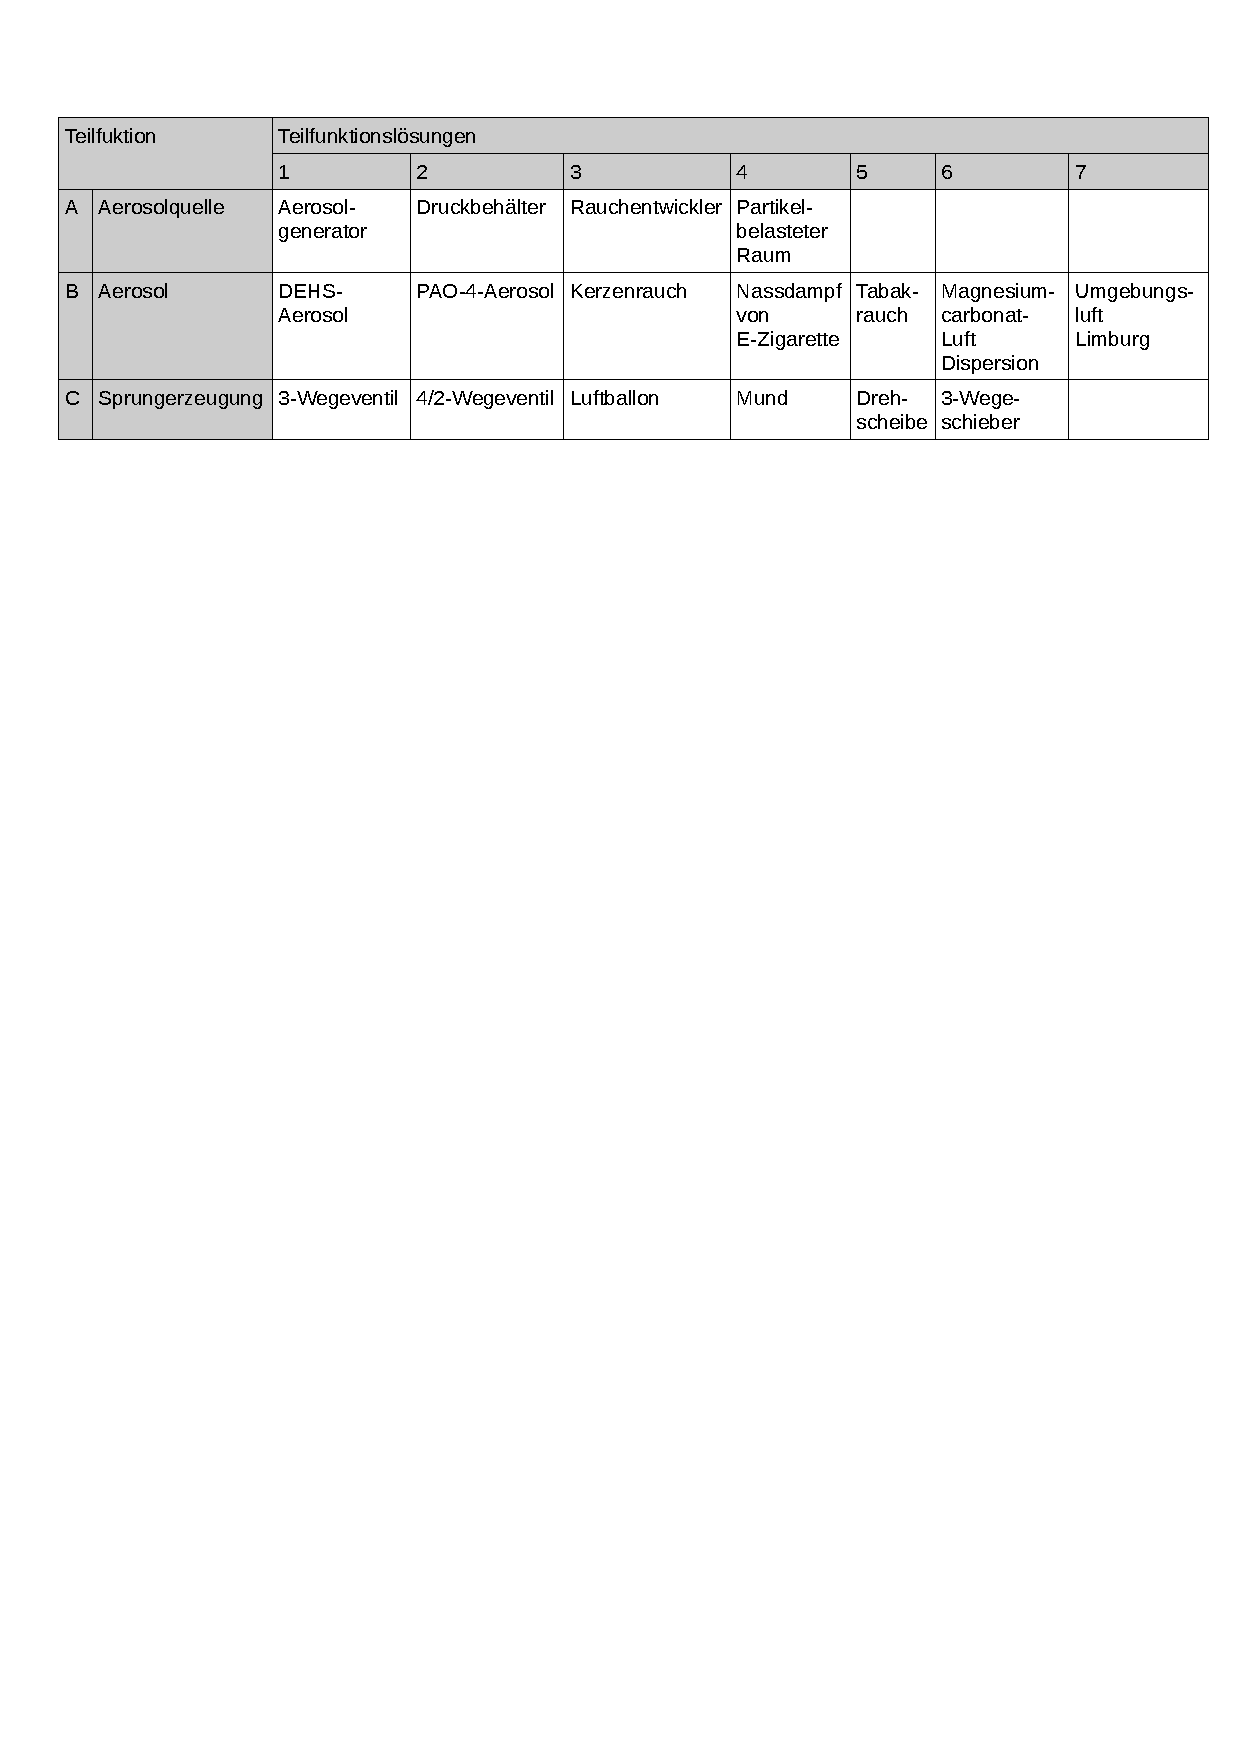
\includegraphics[width=.9\linewidth]{gfx/concepts/Morph.jpg}} \quad
        \caption[Morphologischer Kasten]
        {Morphologischer Kasten}
        \label{fig:Morph}
\end{figure}
Im Falle des OPS 3330 ist nur eine Druckdifferenz zwischen Aerosoleinlass und Messger\"{a}teauslass gegeben, welche den Grenzwert von \(P < 0,756 kPa\) nicht \"{u}berschreiten darf. Somit kann durch den konstruktiven Ma{\ss}nahmen, wie eine dem Auslass in Reihe geschaltete Pumpe, der Aerosolgenerator unabh\"{a}ngig von seinem Betriebsdruck genutzt werden.
\\\\
Bei den Berechnungen des Betriebsdruckes ist zu beachten, dass Druck\"{a}nderungen aufgrund von Leitungsreibung, eventuell horizontal verlaufenden Leitungsabschnitten, Querschnitts\"{u}berg\"{a}ngen, Umlenkungen und zugeschalteten Ger\"{a}ten vorerst vernachl\"{a}ssigt wurden. Au{\ss}erdem wurde angenommen, dass der Aerosolauslass den erforderlichen Volumenstrom bereitstellt, zum Beispiel durch eine Mischstufe mit Umgebungsluft. Genauere Ergebnisse k\"{o}nnen nur durch Betrachtung des fertigen Pr\"{u}faufbaus erfolgen.
\\\\
Zur Nutzung des Aerosolgenerators werden als m\"{o}gliche Aerosole eine DEHS-Luft Dispersion und PAO-4-Luft Dispersion genutzt, da diese den Anforderungen entsprechen und zudem gesundheitlich unbedenklich sind. Als m\"{o}gliche Aerosole f\"{u}r einen Rauchentwickler wurden der Rauch einer Kerzen, Tabakrauch und der Nassdampf einer E-Zigarette in Betracht gezogen. Der Rauch solcher Entwickler besteht aus unterschiedlichen organischen und anorganischen Substanzen, die unterschiedliche Eigenschaften aufweisen. Es besteht somit keine konstante Partikelgr\"{o}{\ss}enverteilung und keine einstellbare Partikelanzahl. Messungen mit Rauchentwicklern sind daher nicht reproduzierbar, da die Gleichheit der Partikeleigenschaften bei erneuten Messungen nicht garantiert werden kann(Q). Die Rauchentwickler erf\"{u}llen die Anforderungen zun\"{a}chst teilweise. Die Partikelgr\"{o}{\ss}en reichen von \(10 nm\) bis zu \(1000 nm\). Jedoch kann nicht sichergestellt werden, dass die Mindespartikelanzahlkonzentration der Partikel, die gr\"{o}{\ss}er als \(500 nm\) sind, f\"{u}r den APS erreicht wird. Hohe Partikelanzahlkonzentrationen ergeben sich f\"{u}r die Partikel der Gr\"{o}{\ss}en \(100 nm\) bis \(450 nm\). Diese Gr\"{o}{\ss}en k\"{o}nnen die anderen Messger\"{a}te erkennen, jedoch ist f\"{u}r diese Ger\"{a}te die Partikelanzahlkonzentration zu hoch.
\begin{align*}
C_\text{Kerze, brennend} < 0,51 - 1,14 * 10^6 \frac{\text{Partikel}}{cm^3}
\end{align*}
\begin{align*}
C_\text{Kerze, ru{\ss}end} < 0,27 - 0,89 * 10^6 \frac{\text{Partikel}}{cm^3}
\end{align*}
\begin{align*}
C_\text{Tabak} > 10^8 \frac{\text{Partikel}}{cm^3}
\end{align*}
\begin{align*}
C_\text{E-Zigarette} > 10^9 \frac{\text{Partikel}}{cm^3}
\end{align*}
Abhilfe kann jedoch durch einen Verd\"{u}nner geschaffen werden. Die Temperatur, die durch den Rauch entsteht, kann mit Hilfe eines Thermokonditionierer geregelt werden.
\\\\
Es besteht zus\"{a}tzlich die M\"{o}glichkeit einen feinstaubbelasteten Raum als Aerosolquelle zu nutzen. Da der ben\"{o}tigte Volumenstrom direkt aus der Umgebung entnommen wird, ist die erforderliche Menge gew\"{a}hrleistet. Auch Luft als Tr\"{a}gergas und die Tr\"{a}gergastemperatur k\"{o}nnen eingehalten werden. Die \"{U}berlegung die Umgebungsluft in Limburg als Aerosol zu nutzen, vereinfacht den Versuchsaufbau. Jedoch liegen Messwerte des hessischen Landesamtes f\"{u}r Naturschutz, Umwelt und Geologie des Jahres 2017 nur f\"{u}r \(PM_{10}\)-Werte vor. Diese liegt bei \(17,3 \frac{\mu g}{m^2}\). Dies entspricht einer Partikelanzahlkonzentration von \(0,033 \frac{\text{Partikel}}{cm^3}\)\cite{hlnug}. Damit ist jedoch nicht sichergestellt, dass die gegebenen Messger\"{a}te alle Partikel erkennen, da die Partikel bis zu \(10 \mu m\) gro{\ss} sein k\"{o}nnen. Durch die \(PM_{10}\)-Wertschwankungen, die tages- und monatsbedingt auftreten, kann die Partikelanzahlkonzentration auch geringer ausfallen. Daher ist die Umgebungsluft als Aerosol unzuverl\"{a}ssig und wird daher ausgeschlossen.\\
In einer Kletterhalle liegt ein hoher Verbrauch von Magnesiumcarbonat vor. In verschiedenen Kletterhallen in Deutschland wurden \(PM_{10}\), \(PM_{2,5}\) und \(PM_1\) Werte gemessen\cite{exp}. Um sicherzustellen, dass die Minimalforderungen eingehalten werden k\"{o}nnen, wurden die Partikelanzahlkonzentration zu den Sto{\ss}zeiten, welche haupts\"{a}chlich abends liegen ausgewertet:
\begin{align*}
C_{PM 1} = 76,39 \frac{\text{Partikel}}{cm^3}
\end{align*}
\begin{align*}
C_{PM 2,5} = 48,89 \frac{\text{Partikel}}{cm^3}
\end{align*}
\begin{align*}
C_{PM 10} = 4,77 \frac{\text{Partikel}}{cm^3}
\end{align*}
Die Mindestpartikelanzahlkonzentration f\"{u}r den FMPS wird nicht erf\"{u}llt. Es wird davon ausgegangen, dass durch den Trendsport die Partikelanzahlkonzentration im Jahre 2018 besonders zu den Sto{\ss}zeiten gestiegen ist, und eine neue Studie n\"{o}tig ist, um die aktuelle Partikeldichte zu messen. Die Studie zeigt, dass die geforderten Partikelgr\"{o}{\ss}en gegeben sind und ein Versuchspr\"{u}fstand mit handels\"{u}blichen Magnesiumcarbonat als Aerosol m\"{o}glich ist. Aufgrund der Nichteignung f\"{u}r den FMPS entf\"{a}llt die Magnesium-Luft Dispersion in einer Kletterhalle als Aerosol.
\\\\
Die Sprungerzeugung ist ein zentraler Mechanismus der Versuchseinrichtung. Daf\"{u}r werden Mehrwegschieber in Betracht gezogen, welche in sp\"{a}teren Kapitel erl\"{a}utert werden. Unkonventionelle Sprungerzeuger in Form eines Luftballons oder mit Hilfe des Mundes entfallen, da sowohl die ben\"{o}tigte menge an Volumenstrom und die erforderliche Mindestmesszeit mit den Partikelsprungerzeugern nicht eingehalten werden kann. Zudem sind die Messungen nicht reproduzierbar.